%----------------------------------------------------------
\subsection*{Задание}\label{blockN.VariantM}
\addcontentsline{toc}{subsection}{Задание}

Даны функция

\begin{equation}
    f(t) = e^{-t^2},\quad t \in [-5;5],
\label{eq:1}
\end{equation}

и функция ошибок

\begin{equation}
    \text{erf }x = \frac{2}{\sqrt{\pi}}\int_{0}^x f(t)dt, \quad x \ge 0.
\end{equation}

\textbf{Требуется (базовая часть)}
\begin{enumerate}
    \item Разработать функцию l(i, x, x\_nodes), которая возвращает значение базисного полинома Лагранжа $l_i(x),$ заданного на узлах с абсциссами x\_nodes, в точке $x$.
    \item Написать функцию L(x, x\_nodes, y\_nodes), которая возвращает значение интерполяционного полинома Лагранжа, заданного на узлах с абсциссами x\_nodes и ординатами y\_nodes, в точке $x$.
    \item Для демонстрации работы функции интерполяции L(x, x\_nodes, y\_nodes) выберите от 5 до 10 произвольных значений некоторой величины и выведите результат работы функции на графике. В качестве интерполируемой величины, на своё усмотрение, можно выбрать любую характеристику, доступную в публичных источниках: статистику температуры воздуха или скорости ветра в городе за несколько дней, курс валют, население страны и пр.
    \item Провести следующий анализ.
    \begin{enumerate}
        \item [а)] Для равномерно расположенных узлов (случай 1) на отрезке $[−5; 5]$ построить графики $f(x)$ и полученных интерполяционных полиномов $L_{n−1}(x)$ для нескольких различных количеств узлов, обозначаемых n. Опишите, что наблюдается при увеличении количества узлов $n$?
        \item [б)] Для каждого $n \in [4, 5. . 20]$ рассчитайте расстояние между $f(x)$ и $L_{n−1}(x)$ в лебеговом пространстве $L_{\infty}$.
        \item [в)] Используя формулу для остаточного члена интерполяции, аналитически оценить верхнюю границу погрешности интерполяции полиномами Лагранжа $L_{n−1}(x)$ в зависимости от $n$. Представить в отчёте в графическом виде сравнение полученного результата с зависимостью расстояния между $f(x)$ и $L_{n−1}(x)$ в лебеговом пространстве $L_{\infty}$ от $n$. Как соотносятся друг с другом полученные аналитическая и численная оценки погрешности аппроксимации?
    \end{enumerate}
    \item Повторить пункт 4 для случая оптимально расположенных узлов (случай 2) и для случая кусочно-линейной интерполяции (случай 3, опциональная часть: аналитическая оценка верхней границы погрешности в общем виде).
    \item Вывести на одном графике зависимости расстояния между $f(x)$ и $L_{n−1}(x)$ в лебеговом пространстве $L_{n−1}(x)$ от $n$ для всех трёх рассмотренных случаев. Как влияет расположение узлов на погрешность аппроксимации? Какое расположение узлов и для каких $n$ даёт более точную интерполяцию? Как влияет использование локальной или глобальной интерполяции на точность интерполяции?
\end{enumerate}

\textbf{Требуется (продвинутая часть)}
\begin{enumerate}
    \setcounter{enumi}{6}
    \item Найти приближённое значение функции ошибок erf $x$ в точке $x = 2$, используя кусочно-линейную интерполяцию для $f(t)$ при $n \in N = \{3, 5, 7, 9\}$ при $t \in [0; 5]$ и сравнить полученные значения между собой.
    \item Представить аналитическое выражение для аппроксимации функции erf $x$, получаемой за счёт использования кусочно-линейной интерполяции $f(t)$ при $n = N_j$, где $N_j$ – $j$-й элемент множества $N$, $j = M \mod{\vert N \vert}+1$, где $M$ – номер обучающегося по журналу.
    \item \textbf{Опциональное задание.} Предложить алгоритм оптимизации кода, который бы позволил сократить число арифметических операций при вычислении значения интерполяционного полинома $L_{n−1}(x)$ в точке $x$. Описать алгоритм в отчёте и обосновать повышение производительности.
\end{enumerate}


%----------------------------------------------------------
\subsection*{Цель выполнения лабораторной работы}
\addcontentsline{toc}{subsection}{Цель выполнения лабораторной работы}

Цель выполнения лабораторной работы: \GoalOfResearch.

%----------------------------------------------------------
\subsection{Реализация функции, возвращающей значение $i$-го базисного полинома Лагранжа в точке $x$}
\label{z1}

По определению\footnote{ссылка на определение} базисный полином $l_i$ при данных $n$ интерполяционных узлах $x_1, x_2,...,x_n$ вычисляется следующим образом:
\begin{equation}
    l_i(x) = \frac{x - x_1}{x_i-x_1}...
    \frac{x - x_{i-1}}{x_i-x_{i-1}}
    \frac{x - x_{i+1}}{x_i-x_{i+1}}...
    \frac{x - x_{n}}{x_i-x_{n}} = \prod_{i \ne j}\frac{x-x_j}{x_i-x_j}.
\label{eq:l_i}
\end{equation}
Формула \eqref{eq:l_i} взята за основу решения поставленной задачи программной реализации.

Здесь и далее использованы язык программирования Python, а также открытые библиотеки NumPy и Matplotlib для вычислений и визуализации данных соответственно, а также модуль стандартной библиотеки math. Во всех листингах подразумевается, что нужные библиотеки и модули уже подключены.

Алгоритм работы функции l(i, x, x\_nodes):
\begin{enumerate}
    \item Создается новый массив x\_nodes\_exc\_i, который содержит все узлы интерполяции исходного массива x\_nodes, исключая $i$-ый узел.
    \item Формируется еще один массив l\_multipliers, внутри которого размещаются значения множителей $\frac{x-x_j}{x_i-x_j}$ из формулы \eqref{eq:l_i}.
    \item Вычисляется произведение элементов массива l\_multipliers.
    \item Полученное на предыдущем этапе значение возвращается из функции.
\end{enumerate}

Листинг 1: Функция, возвращающая значение $i$-го базисного полинома Лагранжа в точке $x$. 
\begin{lstlisting}[label={lst:listing1}]
def l(i, x, x_nodes):
    x_nodes_exc_i = np.r_[x_nodes[:i], x_nodes[i+1:]]
    l_multipliers = (x - x_nodes_exc_i) / (x_nodes[i] - x_nodes_exc_i)
    return np.prod(l_multipliers)
\end{lstlisting}

В результате реализована функция l(i, x, x\_nodes), возвращающая значение $i$-го базисного полинома по заданным параметрам:
\begin{itemize}
    \item i: int
    \quad Номер узла интерполяции.
    \item x: int
    \quad Некоторая точка $x$.
    \item x\_nodes: array\_like
    \quad Множество всех узлов интерполяции.
\end{itemize}

%----------------------------------------------------------
\subsection{Реализация функции, возвращающей значение интерполяционного полинома Лагранжа в точке $x$}
\label{z2}

По аналогии с задачей \ref{z1}, определение\footnote{ссылка на определение} интерполяционного полинома Лагранжа $L_{n-1}(x)$ для функции $f(x)$, заданной в $n$ интерполяционных узлах $x_1, x_2,...,x_n$ на отрезке $[a;b]$ имеет следующий вид:
\begin{equation}
    L_{n-1}(x) = \sum_{i=1}^{n}f(x_i)l_i(x) = \sum_{i=1}^{n}f(x_i)\prod_{i \ne j}\frac{x-x_j}{x_i-x_j},
\label{eq:L}
\end{equation}
где $l_i(x)$ = $\prod_{i \ne j}\frac{x-x_j}{x_i-x_j}$ - базисный многочлен Лагранжа $(n-1)$-й степени.

В основу решения данной задачи легли уравнение \eqref{eq:L} и функция l(i, x, x\_nodes), реализованная в задаче \ref{z1}.

Алгоритм работы функции L(x, x\_nodes, y\_nodes):
\begin{enumerate}
    \item Формируется массив L\_summands, содержащий в себе значенения слагаемыех $f(x_i)l_i(x)$, вычисленных с помощью функции l(i, x, x\_nodes) из задачи \ref{z1}.
    \item Функция numpy.sum\footnote{пояснение функции} вычисляет сумму элементов массива L\_summands.
    \item Полученное на предыдущем этапе значение возвращается из функции.
\end{enumerate}

Листинг 2: Функция, возвращающая значение интерполяционного полинома Лагранжа в точке $x$.
\begin{lstlisting}[label={lst:listing2}]
def L(x, x_nodes, y_nodes):
    L_summands = y_nodes * np.array([l(i, x, x_nodes) for i in range(len(x_nodes))])
    return np.sum(L_summands)
\end{lstlisting}

В результате реализована функция L(x, x\_nodes, y\_nodes), возвращающая значение интерполяционного полинома Лагранжа по заданным параметрам:
\begin{itemize}
    \item x: int
    \quad Некоторая точка $x$.
    \item x\_nodes: array\_like
    \quad Множество всех узлов интерполяции.
    \item y\_nodes: array\_like
    \quad Множество значений всех узлов интерполяции\footnote{$i$-й элемент множества значений должен соответствовать $i$-ому элементу множества узлов}.
\end{itemize}

%----------------------------------------------------------
\subsection{Демонстрация работы функции интерполяции Лагранжа}
\label{z3}

В качестве интерполируемой величины был выбран процент детей, не посещающих начальную школу в России (по годам). Для удобства обозначим зависимость процента детей от года как функцию $bad\_kid\_percent(year)$. Используемые данные взяты из интернет-ресурса по адресу:
\begin{center}
    \href{https://statbase.ru/data/rus-children-out-of-school-percent-of-primary-school-age/}{https://statbase.ru/data/rus-children-out-of-school-percent-.../}.
\end{center}
Конкретные выбранные значения представлены в таблице \ref{tab:table1}.

% \begin{flushright}
% Таблица 1\par
% Выбранные значения для интерполяции\end{flushright}
%\usepackage{caption}

\begin{table}[htbp]
\centering
\captionsetup{singlelinecheck=false}
\caption{\\ Выбранные значения для интерполяции}
\begin{tabular}{ |c|c|c|c|c|c|c|c|c| } 
 \hline
 Год & 2007 & 2008 & 2009 & 2011 & 2012 & 2013 & 2014 & 2015 \\
 \hline
 Дети, не посещающие школу, \% & 6.21 & 4.71 & 4.90 & 4.62 & 2.65 & 2.95 & 2.78 & 0.83 \\ 
 \hline
\end{tabular}
\label{tab:table1}
\end{table}

Для построения графика аппроксимации функции $bad\_kid\_percent(year)$ необходимо вычислить несколько значений интерполяционного полинома Лагранжа в точках, принадлежащих отрезку $[2007;2015]$. Чем больше значений будет рассчитано, тем более гладким будет выглядеть график. По выбранным узлам интерполяции из таблицы \ref{tab:table1} и эмпирически подобранным 200 равномерно расположенным точкам на отрезке $[2007;2015]$, вычислены значения интерполянта функции $bad\_kid\_percent(year)$. Полученные точки отображены на графике посредством инструментов библиотеки Matplotlib. График представлен на рис. \ref{fig:fig1}.

Более структурированно описанный выше алгоритм построения графика некоторой функции $p=p(x)$ на отрезке $[a;b]$ будет выглядеть так:
\begin{enumerate}
    \item Создается массив X равномерно распределенных точек на отрезке $[a;b]$. Количество точек определяется так, чтобы график по возможности выглядел гладким.
    \item Генерируется массив P значений функции $p(x)$ для каждой точки массива X.
    \item По полученным парам $(X_i;P_i)$ строится приближенный график функции $p(x)$.
\end{enumerate}
Данная последовательность действий является стандартной для подобной задачи построения графика, и в дальнейшем будет опускаться или описываться кратко.

\begin{figure}
    \centering
    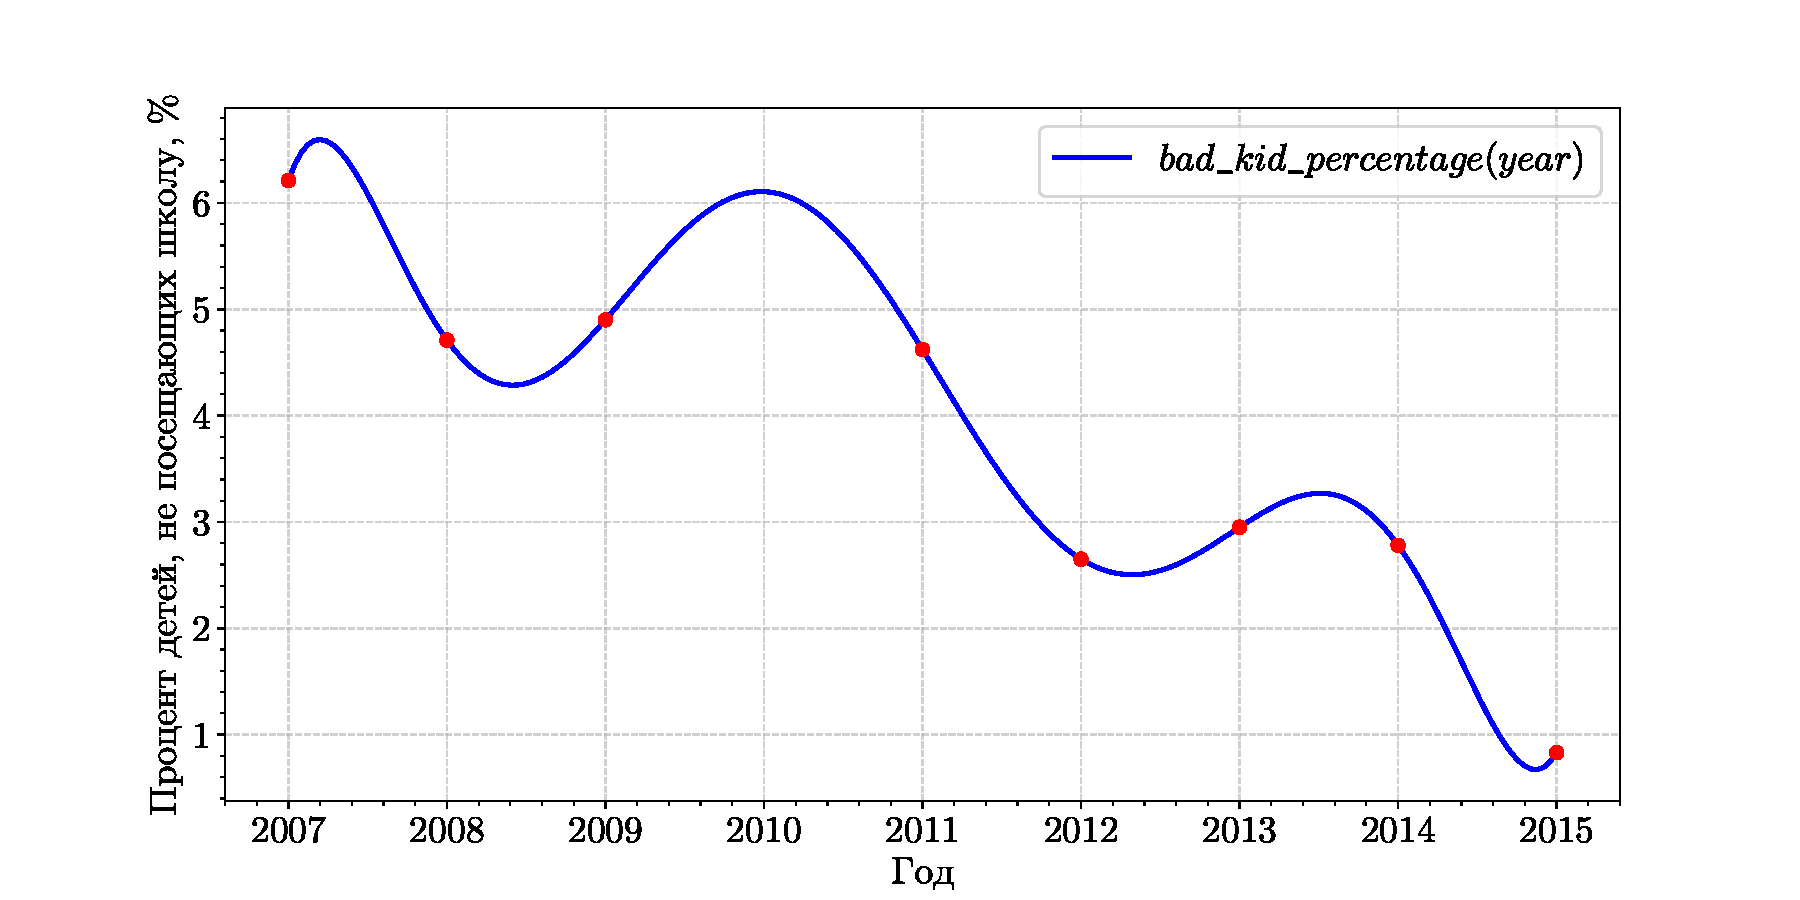
\includegraphics[width=1\linewidth]{labs/kid_percentage_interpolation.pdf}
    \caption{График интерполяционного полинома Лагранжа для функции $bad\_kid\_percent(year)$ (синим) вместе с интерполяционными узлами (красные точки)}
    \label{fig:fig1}
\end{figure}
\pagebreak

%----------------------------------------------------------
\subsection{Анализ зависимости погрешности интерполяции Лагранжа от количества интерполяционных узлов}
\label{z4}

\subsubsection{а) Построение графиков $f(x)$ и $L_{n-1}(x)$ для различных n}
\label{z4a}

Для построения графиков функции \eqref{eq:1} и ее интерполяционных полиномов при разных $n$ была написана функция f(x), принимающая на вход некоторую точку $x$ и возвращающая значения функции \eqref{eq:1} в этой точке. 

Листинг 3: Функция, возвращающая значение функции $f(x) = e^{-x^2}$ в точке $x$.
\begin{lstlisting}[label={lst:listing3}]
def f(x):
    return math.e**(-x**2)
\end{lstlisting}
С ее помощью по описанному ранее в задаче \ref{z3} алгоритму строится график самой функции \eqref{eq:1}. А также графики интерполяционного полинома Лагранжа $L_{n-1}(x)$ для функции \eqref{eq:1} при разных количествах $n$ интерполяционных узлов. Были выбраны значения $n \in [4;6;8;...;20]$ (всего 9 значений). Получившиеся графики представлены на рис. \ref{fig:fig2}.

\begin{figure}
    \centering
    \hspace*{-2em}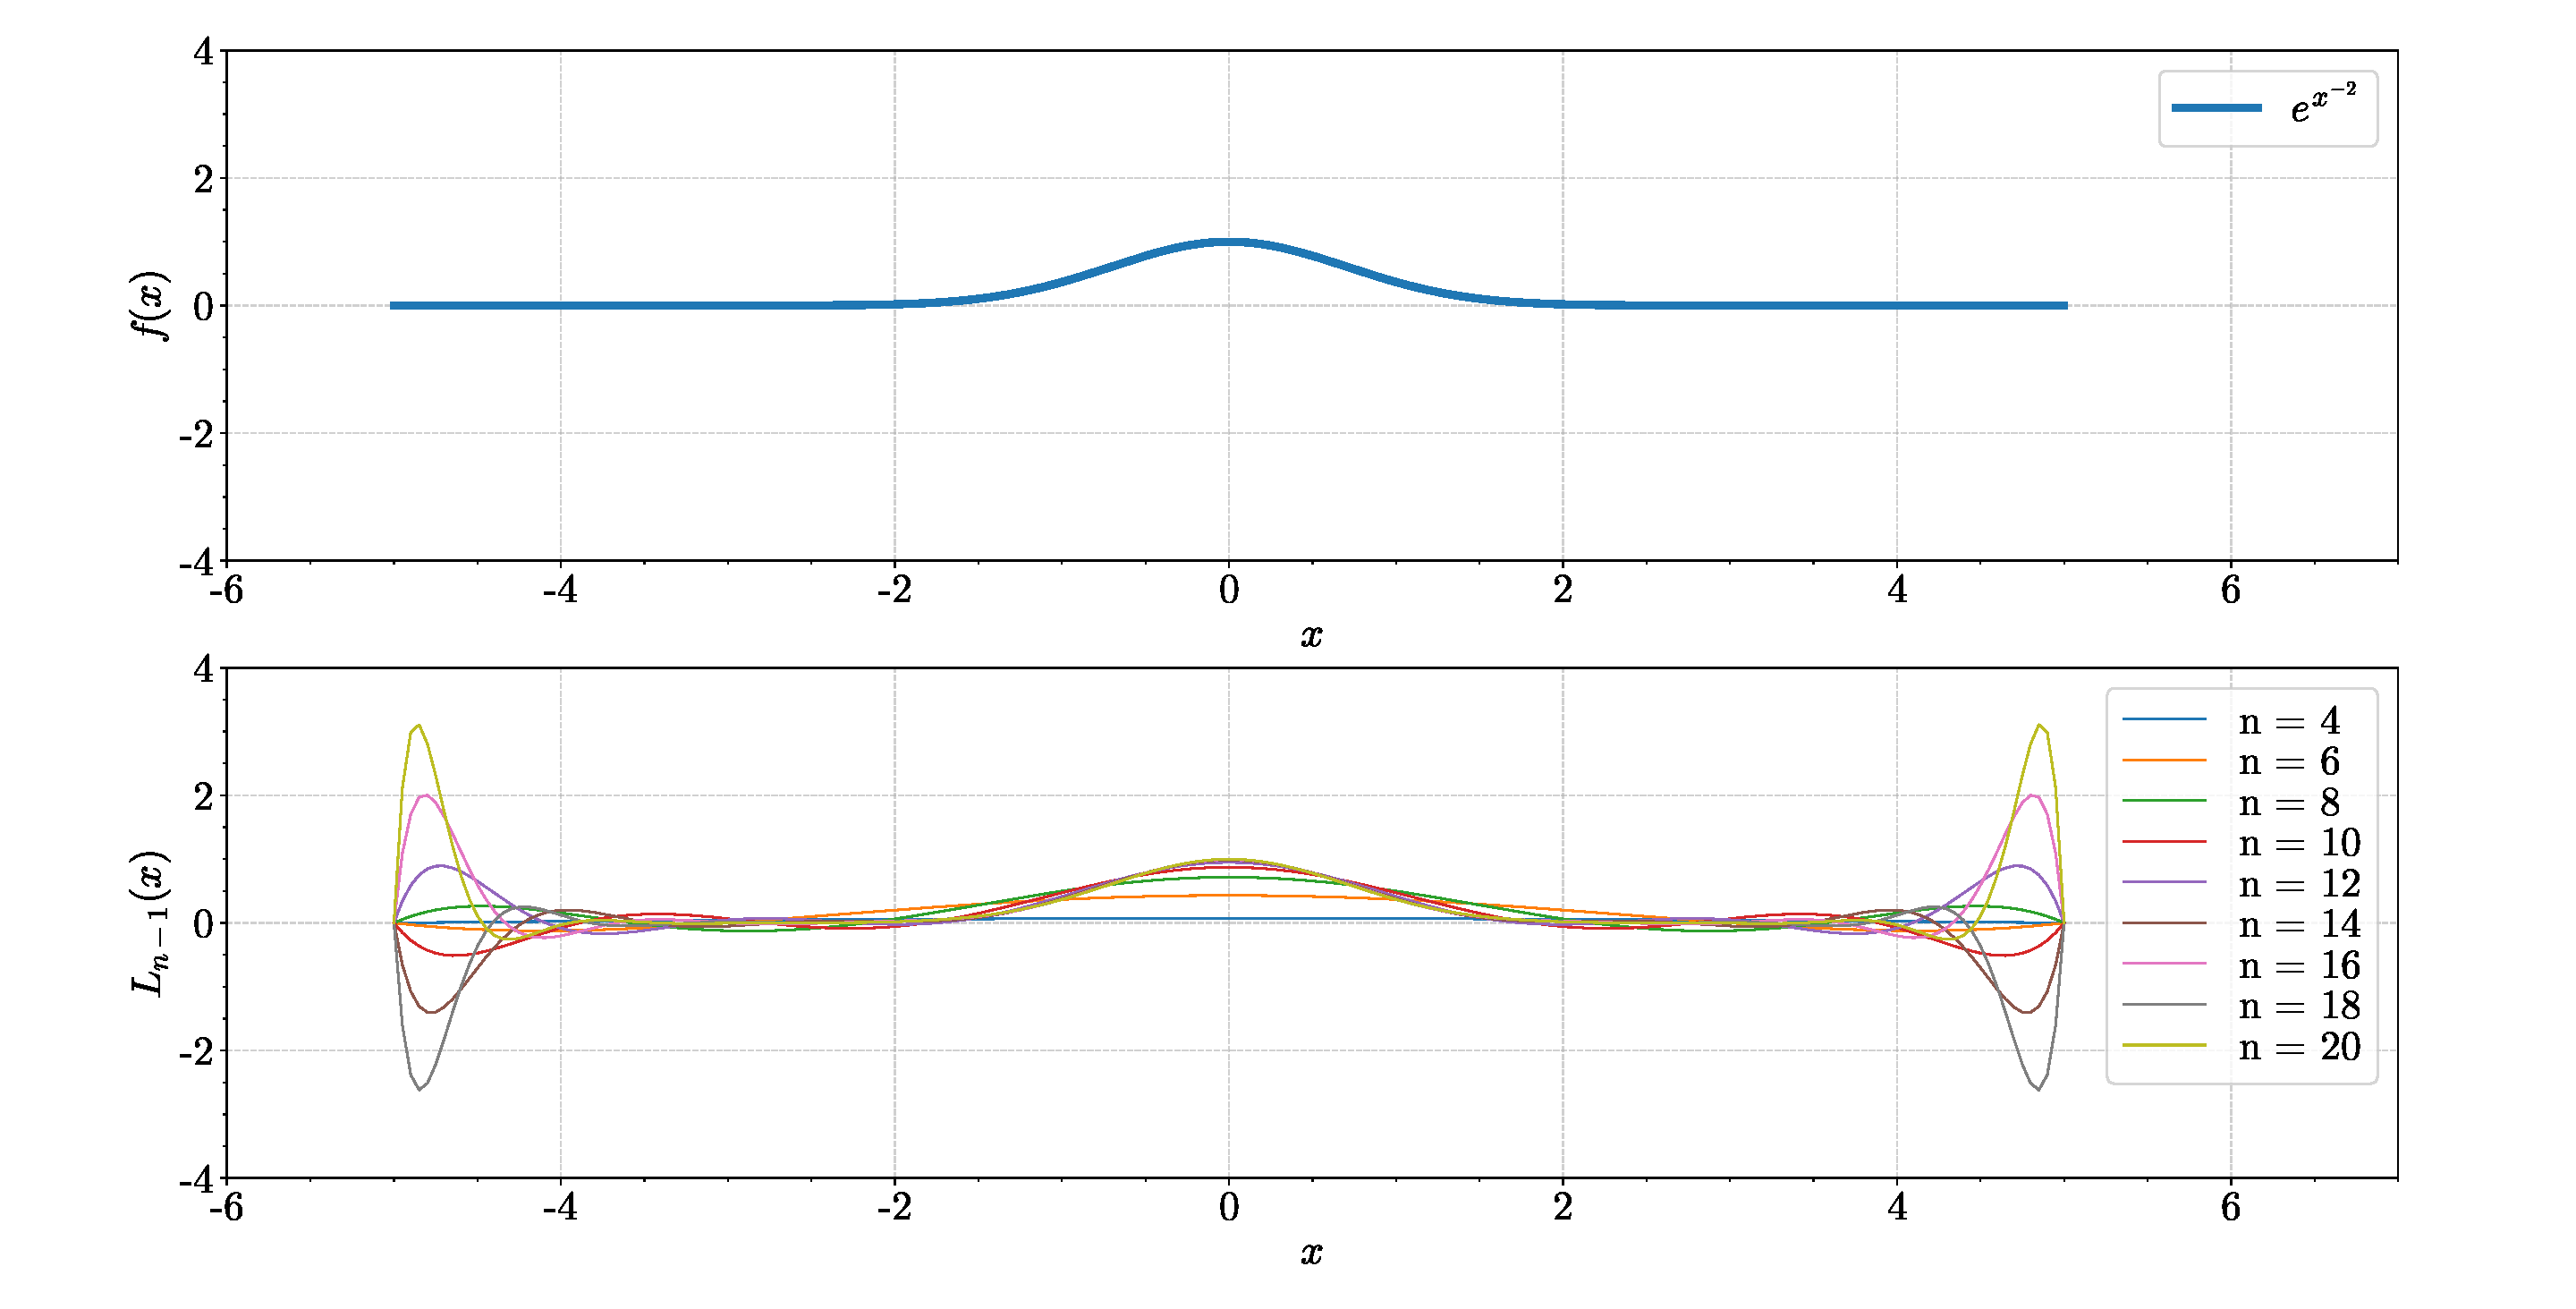
\includegraphics[width=1.1\linewidth]{labs/f(x) + L_n-1.pdf}
    \caption{Графики функции $f(x)$ и ее интерполянта $L_{n-1}(x)$ при различных $n$ на отрезке $x \in [-5;5]$}
    \label{fig:fig2}
\end{figure}

На представленном графике интерполяционного многочлена Лагранжа $L_{n-1}(x)$ для функции \eqref{eq:1} хорошо видно, что с увеличением числа $n$ интерполяционных узлов на краях рассматриваемого отрезка $x \in [-5;5]$ возникают «паразитные» осцилляции — резкие возрастания колебаний интерполяционной кривой. Явление осцилляции относится к нежелательному явлению, так как приводит к увеличению ошибки интерполяции.
\pagebreak

\subsubsection{б) Численный расчет расстояний между $f(x)$ и $L_{n-1}(x)$ в лебеговом пространстве $L_{\infty}$ для различных $n$}
\label{z4b}

В лебеговых пространствах $L_p$ под расстоянием между двумя функциями $g_1 = g_1(x)$ и $g_2 = g_2(x)$ подразумевается норма $||g_1 - g_2||_p$. В пространстве $L_{\infty}$ нормой функции $g(x)$ является равномерная (также Чебышевская) норма
\begin{equation}
    ||g||_{\infty} = \sup_{x \in X}|g(x)|,
\end{equation}
что для $g(x)$, заданной на $x \in [a;b]$ равнозначно
\begin{equation}
    ||g||_{\infty} = \max_{x \in [a;b]}|g(x)|.
\end{equation}

Таким образом, искомые расстояния в пространстве $L_{\infty}$ между функцией \eqref{eq:1} и ее интерполянтами $L_{n-1}(x)$ для $n \in [4,5,...,20]$ при $x \in [-5;5]$ рассчитываются как
\begin{equation}
    ||f(x)-L_{n-1}(x)||_{\infty}=\max_{x \in [-5;5]}|f(x)-L_{n-1}(x)|.
\end{equation}

Для численного расчета расстояний была реализована функция calculate\_max\_distance(y1, y2). Она принимает на вход два массива y1 и y2 — множества значений двух функций, между которыми ищется расстояние, и возвращает это искомое расстояние.
\pagebreak

Листинг 4: Функция, возвращающая расстояние между функциями в лебеговом пространстве $L_{\infty}$.
\begin{lstlisting}[label={lst:listing4}]
def calculate_max_distance(y1, y2):
    distances = abs(y1-y2)
    return max(distances)
\end{lstlisting}

Расчет произведен по следующему алгоритму:
\begin{enumerate}
    \item Создается массив X равномерно расположенных $n$ точек на отрезке [-5;5]. Чем больше 
 количество точек $n$, тем точнее будет рассчитанное расстояние\footnote{На самом деле это не всегда так, но общая закономерность такова}.
    \item Высчитывается массив f\_X, содержащий значения функции \eqref{eq:1} во всех точках массива X.
    \item В цикле для $i$-го количества точек $n \in [4,5,...,20]$ считаются значения интерполирующей функции $L_{n-1}(x)$ в каждой точке массива X, значения записываются в массив L\_X.\label{alg:p3}
    \item При помощи функции calculate\_max\_distance(y1, y2) вычисляется расстояние между функциями \eqref{eq:1} и $L_{n-1}(x)$. Расстояние выводится на экран.\label{alg:p4}
    \item Пункты \ref{alg:p3} и \ref{alg:p4} повторяются для всех точек $n \in [4,5,...,20]$.
\end{enumerate}

Программная реализация данного алгоритма приведена на листинге \hyperref[lst:listing5]{5}.

Листинг 5: Функция, возвращающая расстояние между функциями в лебеговом пространстве $L_{\infty}$.
\begin{lstlisting}[label={lst:listing5}]
    X = np.linspace(-5, 5, 200)
    f_X = np.array([f(x) for x in X])
    
    print('Approximate distances between f(x) and L_n-1(x):')
    
    for n in range(4, 21):
        x_nodes = np.linspace(-5, 5, n)
        y_nodes = np.array([f(x) for x in x_nodes])
        L_X = [L(x, x_nodes, y_nodes) for x in X]
        print(f'At n = {n:<2} equals: {round(calculate_max_distance(f_X, L_X), 3):>.3f}')
\end{lstlisting}

Получившиеся расстояния приведены в таблице \ref{tab:table2}.

\begin{table}[h!]
\caption{\\ Приблизительные расстояния между \( f(x) \) и \( L_{n-1}(x) \)}
\centering
\begin{tabular}{|c|c|}
\hline
Количество узлов $n$ & Расстояние между $f(x)$ и $L_{n-1}(x)$ \\ \hline
4 & 0.929 \\ \hline
5 & 0.560 \\ \hline
6 & 0.568 \\ \hline
7 & 0.891 \\ \hline
8 & 0.284 \\ \hline
9 & 1.485 \\ \hline
10 & 0.512 \\ \hline
11 & 2.329 \\ \hline
12 & 0.892 \\ \hline
13 & 3.373 \\ \hline
14 & 1.403 \\ \hline
15 & 4.524 \\ \hline
16 & 2.003 \\ \hline
17 & 5.575 \\ \hline
18 & 2.617 \\ \hline
19 & 6.393 \\ \hline
20 & 3.106 \\ \hline
\end{tabular}
\label{tab:table2}
\end{table}

Из данных, представленных в таблице \ref{tab:table2} подтверждается, что при увеличении числа интерполяционных узлов $n$, осцилляции, рассмотренные в пункте \hyperref[z4a]{4а}, приводят к увеличению погрешности интерполяции. Также заметно, что при общей тенденции увеличения, расстояние может и уменьшаться относительно нескольких предыдущих меньших значений $n$. Такое поведение связано с самим расположением интерполяционных узлов, которое зависит от их количества.
\pagebreak

\subsubsection{в) Аналитическая оценка верхней границы погрешности интерполяции в зависимости от $n$, сравнение с численной}

О погрешности, возникающей при аппроксимации многочленами Лагранжа $L_{n-1}(x)$ гласит следующая теорема (теорема об остаточном члене многочлена Лагранжа\footnote{ссылка на источник}):
\vspace{5mm}\\
Пусть $x_1, ..., x_n \in [a;b]$ - интерполяционные узлы и $f(x) \in C^n[a;b]$. Тогда $\forall x \in [a;b] \quad \exists \xi \in (a;b)$ такое, что
\begin{equation}
\label{eq:8}
    f(x) - L_{n-1}(x) = \frac{f^{(n)}(\xi)}{n!} \prod_{i = 1}^{n}(x-x_i)
\end{equation}
\vspace{5mm}

И хотя данная теорема в явном виде определяет значение погрешности интерполяции (если взять значение остаточного члена по модулю), но в то же время не сообщает, в каком именно $\xi$ данное равенство будет выполняться. Только говорит о его существовании на интервале $(a;b)$. Поэтому будет оцениваться верхняя граница погрешности, то есть для каждой погрешности будет учитываться максимальное значение $f^{(n)}(\xi)$.

Попробуем аналитически выразить производную $f^{(n)}(\xi)$ для функции \ref{eq:1}. Начнем с вычисления первых нескольких производных:
\vspace{5mm}

\begin{equation*}
    f'(\xi) = \frac{d}{d\xi}(e^{-\xi^2})=-2\xi e^{-\xi^2},
\end{equation*}

\begin{equation*}
    f''(\xi) = \frac{d}{d\xi}(-2\xi e^{-\xi^2}) = (4\xi^2-2)e^{-\xi^2},
\end{equation*}

\begin{equation*}
    f'''(\xi) = \frac{d}{d\xi}((4\xi^2-2)e^{-\xi^2}) = (-8\xi^3+12\xi)e^{-\xi^2}.
\end{equation*}

Из вычислений видно, что каждую производную $f^{(n)}(\xi)$ можно представить в виде произведения
\begin{equation}
    f^{(n)}(\xi)=P_n(\xi)e^{-\xi^2},
\label{eq:9}
\end{equation}
где $P_n(\xi)=\sum_{k=0}^na_k\xi^k$ – некоторый полином степени $n$.

Продифференцировав \eqref{eq:9} еще раз, получим следующую производную $f^{(n+1)}(\xi)$ в общем виде
\begin{equation}
    f^{(n+1)}(\xi)=\frac{d}{d\xi}(f^{(n)}(\xi))=\frac{d}{d\xi}(P_n(\xi)e^{-\xi^2})=P'_n(\xi)e^{-\xi^2}+P_n(\xi)(-2\xi e^{-\xi^2})=e^{-\xi^2}(P'_n(\xi)-2\xi P_n(\xi)),
\label{eq:10}
\end{equation}
\\
эту же производную можно представить и в виде самого произведения \eqref{eq:9}
\begin{equation}
    f^{(n+1)}(\xi)=P_{n+1}(\xi)e^{-\xi^2},
\label{eq:11}
\end{equation}
\\
теперь, подставив \eqref{eq:11} в \eqref{eq:10}
\begin{equation}
    P_{n+1}(\xi)e^{-\xi^2}=e^{-\xi^2}(P'_n(\xi)-2\xi P_n(\xi)),
\label{eq:12}
\end{equation}
\\
и разделив обе части на $e^{-\xi^2}>0$, имеем уравнение
\begin{equation}
    P_{n+1}(\xi)=P'_n(\xi)-2\xi P_n(\xi).
\label{eq:13}
\end{equation}

Уравнение \eqref{eq:13} является рекуррентным соотношением, выражающим полином $P_{n+1}(\xi)$ через предыдущий полином $P_{n}(\xi)$ и его производную. В качестве начального условия служит равенство $P_0(\xi)=1$, так как $f(\xi)$ можно представить как $f(\xi)=1\cdot e^{-\xi^2}$.

Однако, получившаяся формула \eqref{eq:13} не определяет общий вид коэффициентов полинома $P_n(\xi)$. В таком случае можно заметить, что это рекуррентное соотношение очень похоже на рекуррентную формулу для многочленов Эрмита $H_n(x)$ (в физическом определении)\footnote{ссылка на источник}. Действительно, для них рекуррентное соотношение выглядит как\footnote{пояснение про стандартную формулу и свойство}
\begin{equation}
    H_{n+1}(x)=2x H_n(x)-H'_n(x),
    \label{eq:14}
\end{equation}
и почти совпадает с \eqref{eq:13}, но имеет противоположные знаки перед $2xH_n(x)$ и $H'_n(x)$. Польза такого наблюдения заключается в том, что для полиномов Эрмита известна явная формула\footnote{ссылка} многочленов $H_n(x)$, определяющая общий вид их коэффициентов:
\begin{equation}
    H_n(x) = \sum_{j=0}^{\lfloor n/2 \rfloor} (-1)^j \frac{n!}{j! (n-2j)!} (2x)^{n-2j}
\label{eq:15}
\end{equation}

Рассмотрим свойство четности полиномов Эрмита: многочлен $H_n(x)$ четен при четном $n$ и нечетен при нечетном $n$\footnote{ссылка}. Тогда из \eqref{eq:14} при $n \equiv 0 \pmod{2}$ имеем:
\begin{equation}
\label{eq:16}
\begin{aligned}
    & H_{n+1}(-x)=-2x H_n(-x)-H'_n(-x)=-2xH_n(x)-2nH_{n-1}(-x)=\\
    & =-2xH_n(x)+2nH_{n-1}(x)=H'_n(x)-2xH_n(x),
\end{aligned}
\end{equation}
\hfill\\
и при $n \equiv 1 \pmod{2}$:\\
\begin{equation}
\label{eq:17}
\begin{aligned}
    & H_{n+1}(-x)=-2x H_n(-x)-H'_n(-x)=2xH_n(x)-2nH_{n-1}(-x)=\\
    & =2xH_n(x)-2nH_{n-1}(x)=2xH_n(x)-H'_n(x).
\end{aligned}
\end{equation}

Здесь (\eqref{eq:16} и \eqref{eq:17}) было использовано свойство\footnote{ссылка} $H'_n(x)=2nH_{n-1}(x)$ полиномов Эрмита.

Из \eqref{eq:16} и \eqref{eq:17} можно сделать вывод, что:
\begin{equation}
\label{eq:18}
    \begin{cases}
      P_{n+1}(\xi) = H_{n+1}(\xi),\quad n \equiv 0 \pmod{2}         \\
      P_{n+1}(\xi) = -H_{n+1}(\xi),\quad n \equiv 1 \pmod{2}
    \end{cases}\,,
\end{equation}
\\
что равносильно
\begin{equation}
    P_{n+1}(\xi)=(-1)^nH_{n+1}(\xi),
\label{eq:19}
\end{equation}
или
\begin{equation}
    P_{n}(\xi)=(-1)^{n+1}H_{n}(\xi).
\label{eq:20}
\end{equation}

\vspace{5mm}
Подставив \eqref{eq:15} в \eqref{eq:20}, получаем аналитическое выражение полинома $P_{n}(\xi)$, определяющееся как
\begin{equation}
    P_{n}(\xi) = (-1)^{n+1}\sum_{j=0}^{\lfloor n/2 \rfloor} (-1)^j \frac{n!}{j! (n-2j)!} (2\xi)^{n-2j}
\label{eq:21}
\end{equation}

и далее подставив \eqref{eq:21} в \eqref{eq:9}, имеем полную аналитическую формулу для вычисления производной $f^{(n)}(\xi)$:
\begin{equation}
    f^{(n)}(\xi) = [(-1)^{n+1}\sum_{j=0}^{\lfloor n/2 \rfloor} (-1)^j \frac{n!}{j! (n-2j)!} (2\xi)^{n-2j}]\cdot e^{-\xi^2}.
\label{eq:22}
\end{equation}

Для расчета значения функции \eqref{eq:22} была реализована функция f\_xi\_nth\_derivative(xi, n), представленная на листинге \hyperref[lst:listing6]{6}. Она принимает на вход точку xi, в которой ищется значение производной, и порядок производной n. Возвращает значение $n$-ой производной функции \eqref{eq:22} в точке xi.
\pagebreak

Листинг 6: Функция, возвращающая значение $n$-ой производной функции $f^{(n)}(\xi)$ в точке $\xi$.
\begin{lstlisting}[label={lst:listing6}]
def f_xi_nth_derivative(xi, n):
p_n = 0
for j in range(0, n//2):
    p_n += (-1)**(n+1) * ((-1)**j * (math.factorial(n)) / (math.factorial(j)
    * math.factorial(n - 2*j)) * (2*xi)**(n - 2*j))
return p_n * math.e**(-xi**2)
\end{lstlisting}

Численно будет вычисляться и значение остаточного члена многочлена Лагранжа \eqref{eq:8}, оно же – оценка верхней границы погрешности, если взять абсолютное значение. Максимальное значение для \eqref{eq:22} будем также находить численно, рассчитывая значения при помощи функции f\_xi\_nth\_derivative(xi, n) в некотором количестве точек $n$, распределенных на интервале $\xi \in (a;b)$, а затем выбирая наибольшее. С этой целью была реализована функция calculate\_lagrange\_remainder(x, x\_for\_calculating, n), принимающая на вход точку x, в которой рассчитывается остаточный многочлен, массив x\_for\_calculating, который содержит точки для расчета (чем больше точек, тем точнее) и количество узлов n интерполянта. Возвращает функция максимальный по модулю остаточный член \eqref{eq:8} для заданных параметров. Реализация приведена на листинге \hyperref[lst:listing7]{7}.

Листинг 7: Функция, возвращающая максимальное по модулю значение остаточного члена интерполяции по $n$ узлам в точке $x$.
\begin{lstlisting}[label={lst:listing7}]
def calculate_lagrange_remainder(x, x_for_calculating, n):
    max_f_xi = -1
    for xi in x-x_for_calculating:
        if abs(f_xi_nth_derivative(xi, n)) > abs(max_f_xi):
            max_f_xi = f_xi_nth_derivative(xi, n)
    x_nodes = np.linspace(-5, 5, n)
    prod = np.prod([x - x_i for x_i in x_nodes])
    return max_f_xi * prod / math.factorial(n)
\end{lstlisting}

Далее требуется перебрать некоторое количество точек на интервале $(a;b)$, чтобы найти наибольший из максимальных по модулю значений остаточного члена интерполяции для каждого $n \in [4,5,...,20]$ количества интерполяционных узлов. Эти значения сохранить для дальнейшего построения графика зависимости оценки верхней границы от $n$. Программная реализация приведена на листинге \hyperref[lst:listing8]{8}.

\begin{lstlisting}[label={lst:listing8}]
analytical_distances_values = []
x_for_calculating = np.linspace(-5, 5, 200)
for n in range(4, 21):
    max_err = 0
    for x in x_for_calculating:
        max_err = max(max_err, abs(calculate_lagrange_remainder(x, x_for_calculating, n)))
    analytical_distances_values.append(max_err)
\end{lstlisting}

С помощью полученных в пункте \hyperref[z4b]{4б} значений расстояний между $f(x)$ и $L_{n−1}(x)$ в лебеговом пространстве $L_{\infty}$ и рассчитанной оценке верхней границы погрешности, построим график, на котором сравним численный и аналитический методы в зависимости от $n$. График приведен на рисунке \ref{fig:fig3}.

\begin{figure}
    \centering
    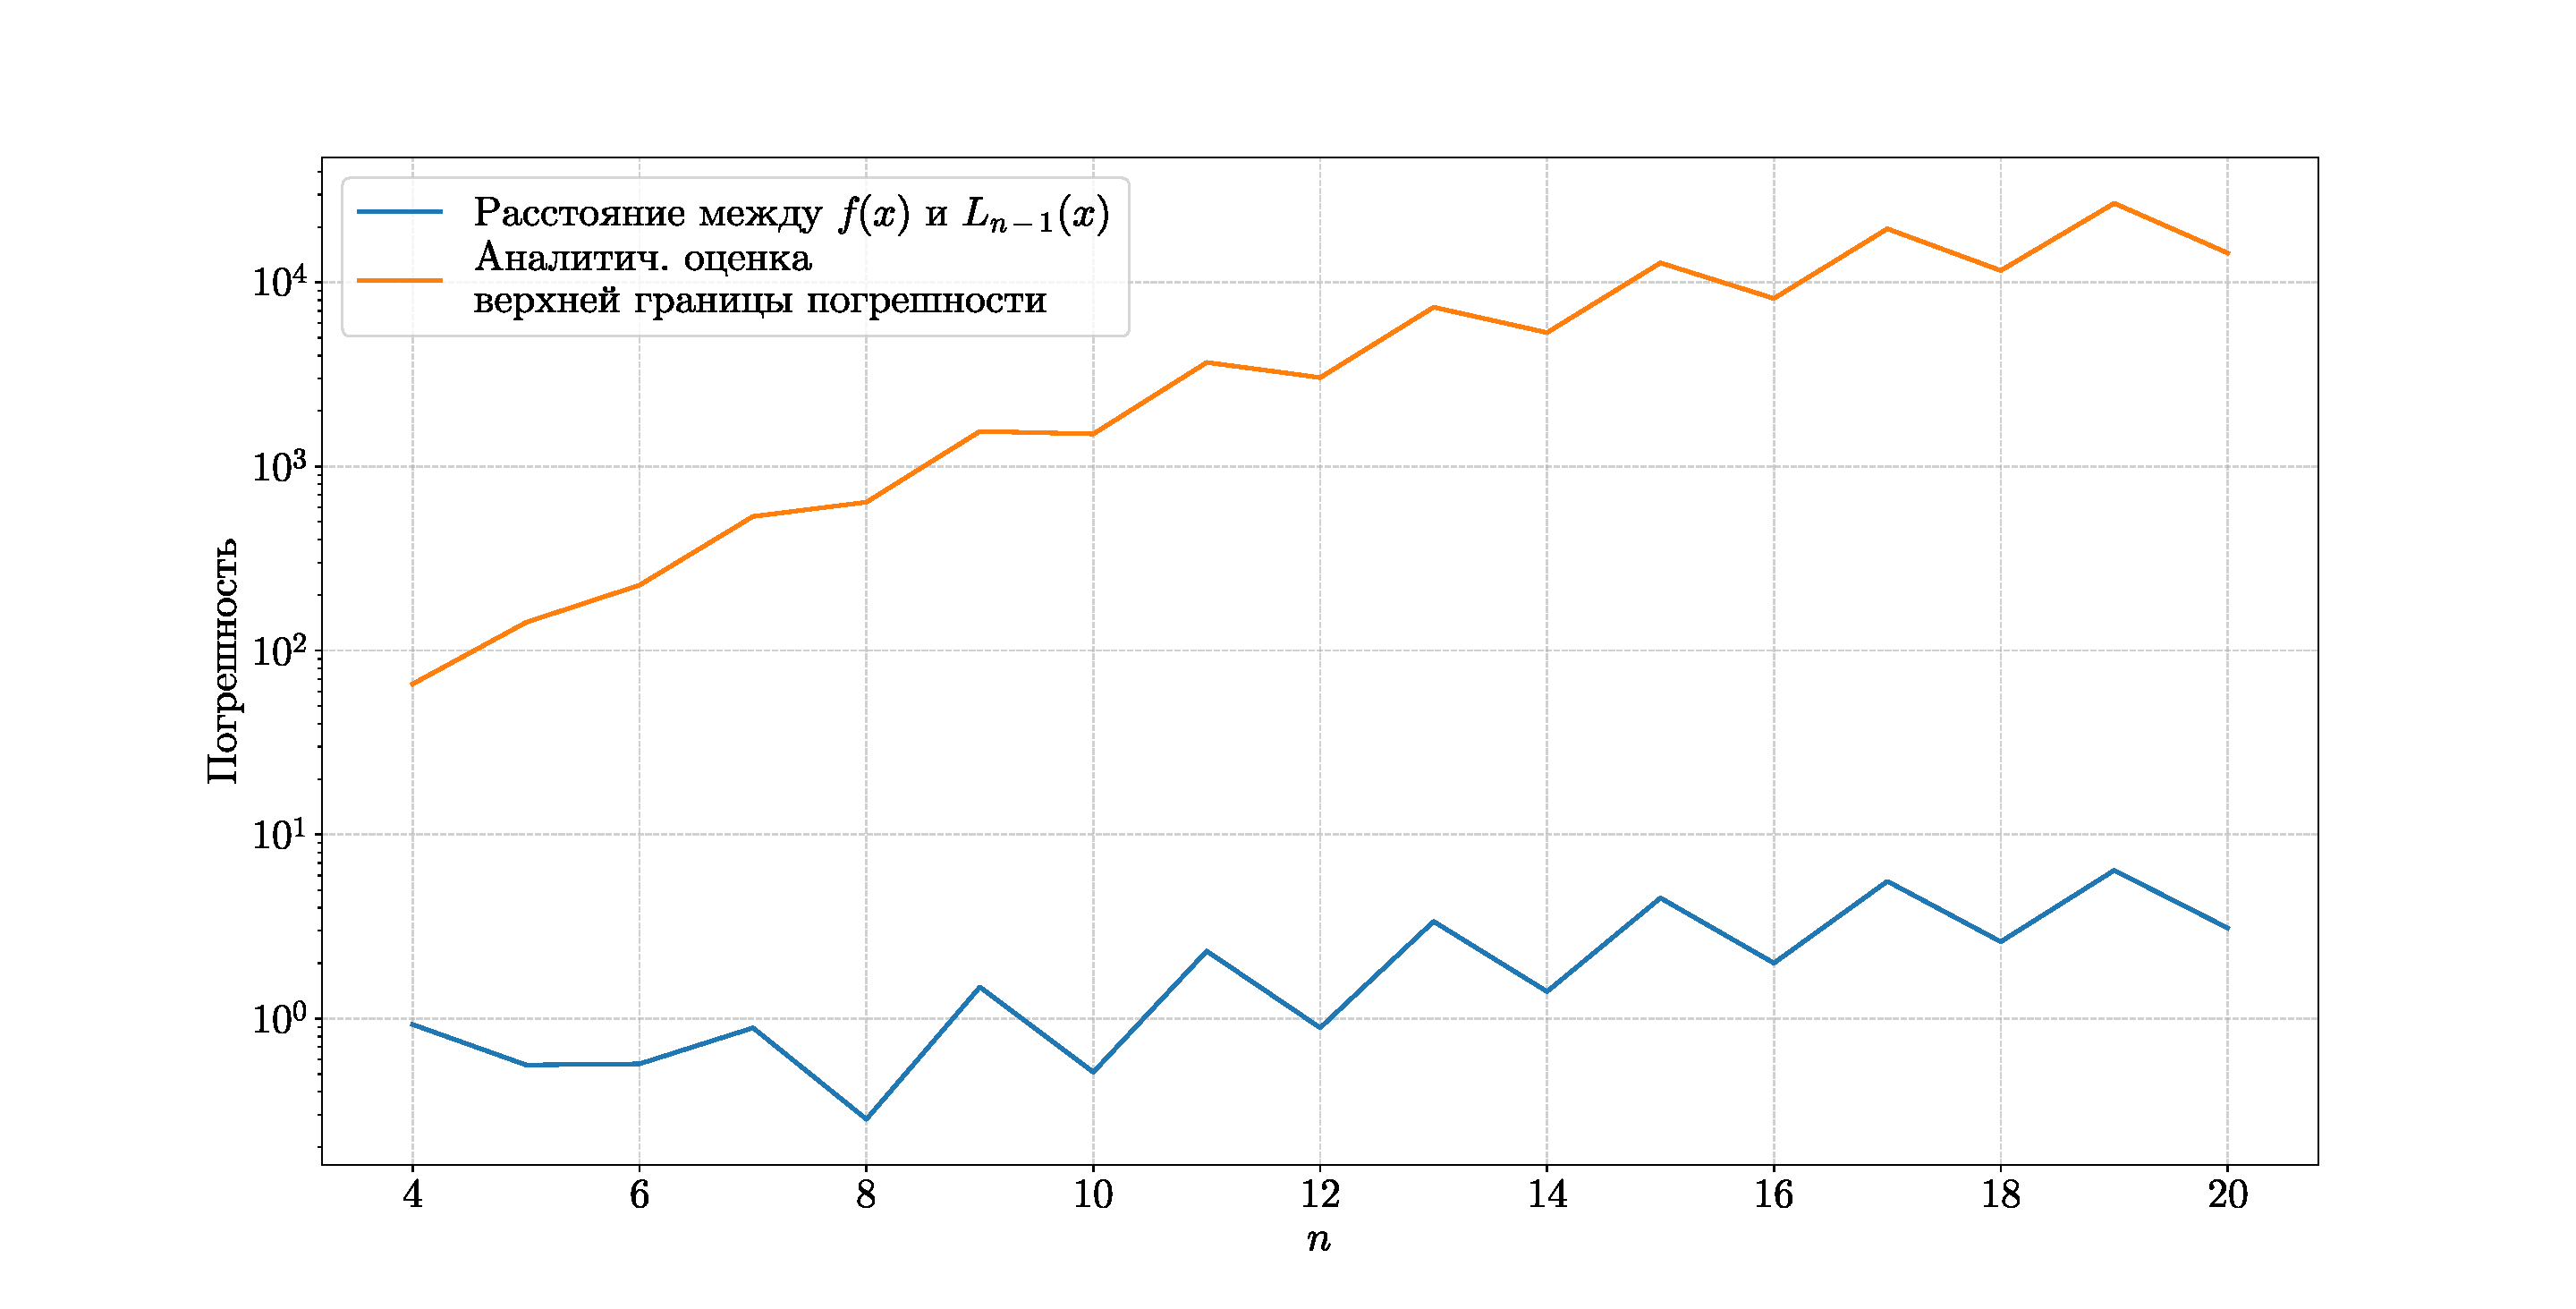
\includegraphics[width=1\linewidth]{labs/approx_vs_analytic.pdf}
    \caption{График расстояния между $f(x)$ и $L_{n−1}(x)$ (синим) и график аналитической оценки верхней границы погрешности при помощи остаточного многочлена Лагранжа (оранжевым) в зависимости от количества интерполяционных узлов $n$}  
    \label{fig:fig3}
\end{figure}

По рисунку \ref{fig:fig3} видно, что аналитическая верхняя граница оказалась больше численной погрешности интерполяции. Это естественно, ведь верхняя граница подразумевает самый худший возможный случай погрешности. Кроме того, снова заметно, что оба графика имеют тенденцию роста с увеличением $n$ ввиду осцилляций, рассмотренных в пункте \hyperref[z4a]{4а}.

%----------------------------------------------------------
\subsection{Повторение анализа для для случая оптимально расположенных узлов и для случая кусочно-линейной интерполяции}

\subsubsection{5.1 Случай оптимально расположенных узлов (случай 2)}
\label{z5a}





\subsubsection{б) Случай кусочно-линейной интерполяции (случай 3)}
\label{z5b}


%----------------------------------------------------------
\subsection{@Название раздела в соответствии с задачей 6@}

\textit{@СОДЕРЖАНИЕ ПОДРАЗДЕЛА@}

%----------------------------------------------------------
\subsection{@Название раздела в соответствии с задачей 7@}

\textit{@СОДЕРЖАНИЕ ПОДРАЗДЕЛА@}

%----------------------------------------------------------
\subsection{@Название раздела в соответствии с задачей 8@}

\textit{@СОДЕРЖАНИЕ ПОДРАЗДЕЛА@}

%----------------------------------------------------------

\subsection*{Заключение}
\addcontentsline{toc}{subsection}{Заключение}

\begin{enumerate}
	\item \textit{@Вывод@}
	\item ...
\end{enumerate}

%----------------------------------------------------------
\subsection*{Список использованных источников}

% Уточнить при подготовке материала
\begin{enumerate}
	\item \bibentry{Pershin2018CompMath}
	\item \bibentry{SokolovPershin2021ManLab}
	\item \bibentry{Sokolov2021ManSem}
	\item \bibentry{Pershin2021CompMathTasks}
	\item \bibentry{PershinSokolov2021CompMathLabs}
%	\item ...
\end{enumerate}

%----------------------------------------------------------
\subsection*{Выходные данные}

\textit{\DocOutReference}
%----------------------------------------------------------
% Атрибуты задачи
\labattributes{}{}{}{}{студент группы \group, \Author}{\Year, \Semestr}
%----------------------------------------------------------

